% Provenance (never printed): see sources/outline_sources.md (Year 3: refraction and
% reflection seismic methods; CMP acquisition, NMO, stacking, Dix; migration in
% principle; seismic stratigraphy). Brief: sources/book5/BRIEFS.md, ch. 2. Curves from
% figdata/bachelor-3/seismic_model.py, refraction_dip.py, synthetic_seismogram.py,
% cmp_nmo.py (the Varden column, region.py); exercise and problem values in the
% Book 5 scratch calculator calc/ch02.py.
\chapter{勘探地震学}\label{ch:b3:exploration-seismology}

一艘勘测船沿海上一条直线缓慢航行，拖曳着一列
气枪，位于水面下几米处，其后还拖着几
千米长、装满水听器的电缆。在提交给监管机构的一次勘测中，
阵列装有 \num{5240} 立方英寸压缩空气，每
\qty{8}{s} 发射一次，震源位于水面下 \qty{12}{m}，窄方位角拖缆
位于此类船只之后，记录的炮检距为 8 至 \qty{10}{km}。
% ledger: noaa5:wg-survey
每次激发都会向海底发出一道声脉冲，下方每一个
岩石界面都会返回一个微弱的回波。经过数周处理后，地质学家
翻看一张剖面图，图中埋藏的古河道、倾斜的断块和
一座古老盆地的\omterm{def:b3:exploration-seismology:terminations}{上超}充填层清晰可见，仿佛地面已被剖开。
上一章的全球尺度地震学利用的是
地震波；勘探地震学则自行产生波源，其时刻与
地点均精确已知，并把记录分布在数千道上。本章
追踪回波从激发到剖面的全过程：折射勘探、
层状地层柱对子波的反射、\omterm{def:b3:exploration-seismology:cmp}{共中心点}方法，
将重复回波转化为速度和清晰图像的方法，偏移
则把反射体放回其应在的位置，以及把剖面作为地层学
来解读。

\begin{recall}
在两种介质的分界面上，声阻抗分别为 $Z_1 = \rho_1v_1$ 和
$Z_2 = \rho_2v_2$，垂直入射的平面波被反射，
反射振幅系数为 $R = (Z_2 - Z_1)/(Z_2 + Z_1)$（
见物理系列本科二年级分册中关于界面处的波）。水平层状折射剖面的首波、截距时间与
交叉距离，已在本科一年级分册讲层状地球的章节中学过；
钻孔柱状图则见第 2 册
（十一年级）。卷积 $(f*g)(t) = \int f(\tau)g(t - \tau)\,\mathrm d\tau$
与傅里叶变换是数学分册的内容。\omterm{def:b3:seismology-imaging:ray-parameter}{射线参数}和
线性\omterm{def:b3:seismology-imaging:inverse}{反演问题}均在\cref{ch:b3:seismology-imaging}中。
\end{recall}

\section{折射勘探}

\begin{definition}[地震折射与反射勘探]\label{def:b3:exploration-seismology:surveys}
\emph{地震折射勘探}\index{地震折射勘探}沿一条检波器测线
记录受控震源的初至，并利用沿较快层顶部传播的
首波求出这些层的速度与深度。
\emph{地震反射勘探}\index{地震反射勘探}在炮检距大多小于
目标深度的条件下记录完整的波列，并利用近似垂直入射的
界面反射波
对地层成像。
\end{definition}

水平层状介质中，首波的到时为 $t = x/v_2 + t_i$，是一条直线，
其斜率给出折射层的速度 $v_2$，其截距 $t_i$
给出折射层的深度。倾斜的折射层使这条直线倾斜：
沿下倾方向激发的首波到时越来越晚，因为折射层越来越深，看起来速度偏慢；
沿上倾方向激发则显得偏快。沿同一测线双向激发，
即反向剖面，可将速度与倾角分开。

\begin{theorem}[倾斜界面上的折射]\label{thm:b3:exploration-seismology:dipping}
速度为 $v_1$ 的层覆盖在速度为 $v_2 > v_1$ 的平面折射层之上，该折射层
沿剖面以角度 $\theta$ 倾斜；$i_c = \arcsin(v_1/v_2)$，$h$ 为
震源正下方折射层的垂直深度。超过临界
距离后，首波的到时为
\begin{align*}
  t &= \frac{x\sin(i_c + \theta)}{v_1} + \frac{2h\cos i_c}{v_1}
  &&\text{沿下倾方向激发},\\
  t &= \frac{x\sin(i_c - \theta)}{v_1} + \frac{2h\cos i_c}{v_1}
  &&\text{沿上倾方向激发}.
\end{align*}
视速度 $v_d = v_1/\sin(i_c + \theta)$ 与
$v_u = v_1/\sin(i_c - \theta)$，由反向剖面可得
\[
  i_c = \tfrac12\left[\arcsin\frac{v_1}{v_d} + \arcsin\frac{v_1}{v_u}\right],\qquad
  \theta = \tfrac12\left[\arcsin\frac{v_1}{v_d} - \arcsin\frac{v_1}{v_u}\right],
  \qquad v_2 = \frac{v_1}{\sin i_c} .
\]
\end{theorem}

\begin{proof}
将坐标系旋转，使折射层水平；此时地表以
$\theta$ 倾斜。沿下倾方向激发时，炮检距为 $x$ 的检波器正下方的垂直深度为
$h + x\sin\theta$，它在折射层上的投影为
$x\cos\theta$。首波路径以临界角 $i_c$ 向下传播至
法线方向，沿折射层以 $v_2$ 传播，再以 $i_c$ 向上。其时间为
\[
  t = \frac{h}{v_1\cos i_c} + \frac{x\cos\theta - h\tan i_c - (h + x\sin\theta)\tan i_c}{v_2}
  + \frac{h + x\sin\theta}{v_1\cos i_c}.
\]
利用 $1/v_2 = \sin i_c/v_1$ 及 $1/\cos i_c - \sin i_c\tan i_c = \cos i_c$，
含 $h$ 的项给出 $2h\cos i_c/v_1$，含 $x$ 的项则给出
$x(\sin i_c\cos\theta + \cos i_c\sin\theta)/v_1 = x\sin(i_c + \theta)/v_1$。
沿上倾方向激发时，$\theta$ 变号。末尾公式由两个
视速度反解出各量。
\end{proof}

反向剖面的两支在两炮点之间须给出相同的时间，
无论由哪一端激发：这就是\emph{互易时间}，是对拾取的检验。
两种情况会使该方法失效。速度比其上层更慢的一层
（速度倒转）不产生首波，因而不可见：其岩石
被计入上方层，其下所有深度都被高估。速度比上层快却
但过薄的层可能永远得不到初至，因为
更深、更快的层的首波追上了它：这便是隐藏层。反射勘探
两者都能看到。

\begin{omfigure}
\begin{tikzpicture}
\begin{axis}[omrecord, width=0.82\linewidth, height=0.46\linewidth,
  xmin=0, xmax=1200, ymin=0, ymax=660,
  xlabel={沿排列的位置，自炮点 W 起算 (\unit{m})},
  ylabel={时间 (\unit{ms})}, legend pos=north west, legend cell align=left,
  legend style={font=\scriptsize}]
\addplot[gray, thick, densely dashed] table[x=x, y=tdir] {figdata/out/bachelor-3-refraction_dip-west.dat};
\addlegendentry{直达波（$v_1$）}
\addplot[blue!70!black, thick] table[x=x, y=thead] {figdata/out/bachelor-3-refraction_dip-west.dat};
\addlegendentry{来自 W 端的首波，沿上倾方向激发}
\addplot[red!70!black, thick] table[x expr=1200-\thisrow{x}, y=thead] {figdata/out/bachelor-3-refraction_dip-east.dat};
\addlegendentry{来自 E 端的首波，沿下倾方向激发}
\addplot[gray, thick, densely dashed, forget plot] table[x expr=1200-\thisrow{x}, y=tdir] {figdata/out/bachelor-3-refraction_dip-east.dat};
\addplot[only marks, mark=*, mark size=1.5pt] coordinates {(1200,486.13) (0,486.13)};
\node[font=\scriptsize, anchor=south east] at (axis cs:1190,530) {互易时间};
\end{axis}
\end{tikzpicture}

\par\smallskip{\small 瓦尔登背斜西翼的反向折射剖面
（计算结果；习题第一部分）。折射面，即石灰岩顶面，
在 \qty{1200}{m} 的观测排列下由 W 向 E 以 \ang{10.8} 抬升；
其上的白垩与页岩合并为一层，速度为 \qty{2.40}{km.s^{-1}}。
自 W 端沿上倾方向激发的首波视速度较快，为 \qty{6.57}{km.s^{-1}}，
自 E 端沿下倾方向激发的首波视速度较慢，为 \qty{3.52}{km.s^{-1}}；两者穿越
整个排列均需 \qty{486.1}{ms}。首波仅在远端附近才
超过直达波，对于如此短的排列，折射面埋藏很深。}
\label{fig:b3:exploration-seismology:refraction}
\end{omfigure}

\section{垂直入射下的反射}

\begin{definition}[地震子波，里克子波]\label{def:b3:exploration-seismology:wavelet}
\emph{地震子波}\index{地震子波}是由震源与记录系统送入地下的
短脉冲，持续几十毫秒；每个反射体返回的都是它的一个按比例缩放的副本。
\emph{里克
子波}\index{里克子波}是峰值频率为 $f$ 的零相位脉冲：
\[
  w(t) = \left(1 - 2\pi^2f^2t^2\right)e^{-\pi^2f^2t^2},
\]
它是高斯函数的二阶导数（相差符号与比例因子）：中央为一个峰，
两侧为两个旁瓣，均值为零，振幅谱在 $f$ 处取最大值。
\end{definition}

\begin{definition}[反射系数序列]\label{def:b3:exploration-seismology:synthetic}
层状地层柱的\emph{反射系数序列}\index{反射系数序列}是
各界面的垂直入射反射系数 $r_k$ 构成的序列，
它们位于各自的双程垂直时间 $\tau_k = \sum_{i \le k} 2h_i/v_i$ 处，即
$r(t) = \sum_k r_k\,\delta(t - \tau_k)$。
\end{definition}

\begin{proposition}[卷积模型]\label{prop:b3:exploration-seismology:synthetic}
若只保留一次反射（不计多次波），且为垂直入射，
不计透射损失、衰减与扩散，且子波 $w$ 不随深度变化，
则记录道是子波与
\omterm{def:b3:exploration-seismology:synthetic}{反射系数序列}的卷积：
\[
  s(t) = \sum_k r_k\,w(t - \tau_k) = (w*r)(t) .
\]
由钻孔测井的速度与密度曲线按此方法算得的记录道，即为该测井的
\emph{合成地震记录}\index{合成地震记录}。
\end{proposition}

\begin{proof}
每个界面返回一份入射子波的副本，其幅度按该界面的系数缩放，
并延迟其双程时间；记录过程是线性的，因此各副本相加。
和式即为 $w$ 与加权狄拉克冲激序列
$r(t)$ 的卷积，由于 $w*\delta(\cdot - \tau_k) = w(\cdot - \tau_k)$。
\end{proof}

\omterm{prop:b3:exploration-seismology:synthetic}{合成地震记录}用于将钻孔与地震剖面相对应：
剖面上的一个反射，与测井曲线中产生该反射的界面相对应。
习题中向斜轴下方的瓦尔登地层柱（即本章的地震模型，
速度与密度在已发表的取值范围内选取，各岩石
分别取值）
% ledger: mavko:velocities
给出下图。白垩–页岩界面仅反射
\qty{2.8}{\percent} 的振幅，因为白垩与页岩
的阻抗几乎相同；石灰岩顶面反射 \qty{38}{\percent}，
石灰岩底面返回一个反向脉冲，基底则返回
一个较强的正脉冲。

\begin{omfigure}
\begin{tikzpicture}
\begin{groupplot}[group style={group size=3 by 1, horizontal sep=0.45cm, y descriptions at=edge left},
  width=0.36\linewidth, height=0.6\linewidth, y dir=reverse, ymin=0.4, ymax=0.85,
  tick label style={font=\scriptsize}, label style={font=\small}, title style={font=\small}]
\nextgroupplot[title={阻抗}, xlabel={\scriptsize $10^6$\,\unit{kg.m^{-2}.s^{-1}}},
  ylabel={双程时间（\unit{s}）}, xmin=4, xmax=14]
\addplot[black, thick] table[x=imp, y=t] {figdata/out/bachelor-3-synthetic_seismogram-log.dat};
\node[font=\tiny, anchor=west] at (axis cs:5.1,0.45) {白垩};
\node[font=\tiny, anchor=west] at (axis cs:5.4,0.535) {页岩};
\node[font=\tiny, anchor=east] at (axis cs:11.6,0.62) {石灰岩};
\node[font=\tiny, anchor=west] at (axis cs:7.0,0.70) {砂岩};
\node[font=\tiny, anchor=east] at (axis cs:13.1,0.79) {片岩};
\nextgroupplot[title={反射系数}, xmin=-0.45, xmax=0.45, xtick={-0.4,0,0.4}]
\addplot[xcomb, red!70!black, thick, mark=*, mark size=1.2pt] table[x=r, y=t] {figdata/out/bachelor-3-synthetic_seismogram-refl.dat};
\draw[gray] (axis cs:0,0.4) -- (axis cs:0,0.85);
\nextgroupplot[title={合成道}, xmin=-0.45, xmax=0.45, xtick={-0.4,0,0.4}]
\addplot[blue!70!black, thick] table[x=s, y=t] {figdata/out/bachelor-3-synthetic_seismogram-trace.dat};
\draw[gray] (axis cs:0,0.4) -- (axis cs:0,0.85);
\end{groupplot}
\end{tikzpicture}

\par\smallskip{\small 向斜轴下方瓦尔登地层柱的\omterm{prop:b3:exploration-seismology:synthetic}{合成地震记录}
（计算结果）。左图：各层阻抗随双程
时间的变化。中图：\omterm{def:b3:exploration-seismology:synthetic}{反射系数序列}，每个界面一条尖峰（
茎线指向右侧表示阻抗增加）。右图：二者与一个
\qty{30}{Hz} 的\omterm{def:b3:exploration-seismology:wavelet}{里克子波}的卷积。每个反射都是子波的副本；微弱的
白垩–页岩反射（位于 \qty{0.488}{s}）几乎不可见。}
\label{fig:b3:exploration-seismology:synthetic}
\end{omfigure}

反射仍能分辨多薄的地层？地层的顶面与底面各返回一个子波，
二者重叠时便发生干涉。

\begin{definition}[调谐厚度]\label{def:b3:exploration-seismology:resolution}
岩层的\emph{调谐厚度}\index{调谐厚度}是指这样一个厚度：
在此厚度下，岩层顶面与底面的反射（符号相反）发生
最强的相长干涉，合成振幅达到最大。更薄的岩层
无法被分辨：其顶面与底面不能再分别拾取，
振幅随厚度成比例减小。
\end{definition}

\begin{proposition}[四分之一波长规则]\label{prop:b3:exploration-seismology:tuning}
对于主周期为 $T$ 的子波，在速度为 $v$ 的岩层中，其反射
系数在顶面为 $+R$、底面为 $-R$，合成反射
在岩层厚度为 $b = \lambda/4$ 时最强，其中 $\lambda = vT$；当
$b \ll \lambda/4$ 时，其振幅与 $b$ 成正比。
\end{proposition}

\begin{proof}
将子波用其主谐波 $\cos(2\pi t/T)$ 表示，两个反射
分别为 $R\cos(2\pi t/T) - R\cos(2\pi(t - \Delta t)/T)$，其中
$\Delta t = 2b/v$，其振幅为 $2R|\sin(\pi\Delta t/T)|$：在
$\Delta t = T/2$ 时最大，即 $b = vT/4$；当 $\Delta t$ 较小时，
振幅约为 $2\pi R\Delta t/T = 4\pi Rb/\lambda$。
\end{proof}

\omterm{def:b3:exploration-seismology:wavelet}{里克子波}并非谐波，其\omterm{def:b3:exploration-seismology:resolution}{调谐厚度}由下图的楔形模型读出，
略小于峰值频率所对应波长的四分之一：
即在 \qty{30}{Hz} 时为 \qty{19.5}{m}，岩\omterm{def:b3:exploration-seismology:velocities}{层速度}为
\qty{3000}{m.s^{-1}}，此时 $\lambda/4 = \qty{25}{m}$。来自千米深度的地震数据，
很少含有高于几十赫兹的显著能量，因为
岩石会吸收高频成分；厚度小于约 \qty{20}{m} 的岩层，
只表现为单一反射。

\begin{omfigure}
\begin{tikzpicture}
\begin{axis}[omrecord, width=0.74\linewidth, height=0.42\linewidth,
  xmin=0, xmax=80, ymin=0, ymax=1.8,
  xlabel={岩层厚度 $b$ (\unit{m})}, ylabel={峰值振幅 / $R$}]
\addplot[blue!70!black, thick] table[x=b, y expr=2*\thisrow{amp}] {figdata/out/bachelor-3-synthetic_seismogram-wedge.dat};
\draw[red!70!black, densely dashed] (axis cs:19.5,0) -- (axis cs:19.5,1.6);
\node[font=\scriptsize, anchor=south, red!70!black] at (axis cs:19.5,1.6) {调谐厚度，\qty{19.5}{m}};
\draw[gray, densely dotted] (axis cs:25,0) -- (axis cs:25,1.6);
\node[font=\scriptsize, anchor=west, gray!40!black] at (axis cs:25.5,0.3) {$\lambda/4 = \qty{25}{m}$};
\draw[gray] (axis cs:0,1) -- (axis cs:80,1);
\node[font=\scriptsize, anchor=south east] at (axis cs:79,1) {两个独立子波};
\end{axis}
\end{tikzpicture}

\par\smallskip{\small 楔形模型（计算结果）：速度为
\qty{3000}{m.s^{-1}} 的岩层，顶面反射系数为 $+R$，底面为 $-R$，
用 \qty{30}{Hz} 的\omterm{def:b3:exploration-seismology:wavelet}{里克子波}成像。合成反射的峰值振幅，
相对于反射系数为 $R$ 的单一反射，在极薄的岩层中从零线性增大，
在\omterm{def:b3:exploration-seismology:resolution}{调谐厚度}处达到峰值，并在厚岩层中趋于
两个独立子波的水平。}
\label{fig:b3:exploration-seismology:wedge}
\end{omfigure}

在横向上，分辨率由能同相送回能量的
反射体的宽度决定。

\begin{definition}[菲涅耳带]\label{def:b3:exploration-seismology:fresnel}
反射体的（第一）\emph{菲涅耳带}\index{菲涅耳带}，指对于位于其上方高度为
$z$ 处、震源与检波器重合的情形，反射体上以法线入射点为中心的圆盘，
该圆盘上的点满足双程路径比法线路径长出的部分
小于半个波长。这些点的反射同相到达，
共同构成记录到的反射。
\end{definition}

\begin{proposition}[菲涅耳带半径]\label{prop:b3:exploration-seismology:fresnel}
第一\omterm{def:b3:exploration-seismology:fresnel}{菲涅耳带}的半径为
$r_F = \sqrt{\lambda z/2 + \lambda^2/16} \approx \sqrt{\lambda z/2}$，适用于
$\lambda \ll z$。
\end{proposition}

\begin{proof}
反射体上与法线入射点距离为 $r$ 的一点，
到震源的距离为 $\sqrt{z^2 + r^2}$。双程多出的路径为
$2(\sqrt{z^2 + r^2} - z)$；令其等于 $\lambda/2$，得
$\sqrt{z^2 + r^2} = z + \lambda/4$，从而 $r^2 = \lambda z/2 + \lambda^2/16$。
\end{proof}

在深度 \qty{1}{km}、$\lambda = \qty{100}{m}$ 时，\omterm{def:b3:exploration-seismology:fresnel}{菲涅耳带}
半径为 \qty{225}{m}：比它窄的构造会被涂抹，除非
下文的\omterm{def:b3:exploration-seismology:migration}{地震偏移}能使\omterm{def:b3:exploration-seismology:fresnel}{菲涅耳带}收缩。

\begin{omfigure}
\begin{tikzpicture}[font=\small, x=1cm, y=1cm]
\fill[brown!12] (-4.5,-3.6) rectangle (4.5,-3.0);
\draw[thick] (-4.5,-3.0) -- (4.5,-3.0);
\node[anchor=north west] at (-4.4,-3.05) {反射体};
\draw[thick] (-4.5,0) -- (4.5,0);
\fill (0,0) circle (2.2pt) node[above] {震源与检波器};
\draw[->, thick] (0,0) -- (0,-2.97);
\node[anchor=west] at (0.05,-1.5) {$z$};
\draw[blue!70!black, thick] (0,0) -- (1.9,-3.0);
\draw[blue!70!black, thick] (0,0) -- (-1.9,-3.0);
\node[anchor=west, blue!70!black] at (1.0,-1.2) {$z + \lambda/4$};
\fill[red!25, opacity=0.7] (-1.9,-3.08) rectangle (1.9,-2.92);
\draw[red!70!black] (0,-3.65) -- (0,-3.95) (1.9,-3.1) -- (1.9,-3.95);
\draw[<->, red!70!black] (0,-3.85) -- (1.9,-3.85) node[midway, below] {$r_F$};
\draw[gray, densely dashed] (-57.6:3.55) arc (-57.6:-122.4:3.55);
\end{tikzpicture}

\par\smallskip{\small 第一\omterm{def:b3:exploration-seismology:fresnel}{菲涅耳带}（示意图）：反射体上，其到重合的
震源与检波器的距离比法线距离 $z$ 多出不足 $\lambda/4$ 的部分
（虚线圆弧：半径为 $z + \lambda/4$ 的球面），因此双程
多出的路径不足半个波长，
其回波同相到达。图中 $\lambda$ 的比例被夸大。}
\label{fig:b3:exploration-seismology:fresnel}
\end{omfigure}

\section{共中心点采集与处理}

单次回波在噪声中太弱，难以辨认。因此反射测量
会以不同的震源–检波器对多次记录每一地下点，
再将记录相加。

\begin{definition}[共中心点，覆盖次数]\label{def:b3:exploration-seismology:cmp}
设测线上震源位于 $x_s$、检波器位于 $x_r$，则中点为
$(x_s + x_r)/2$，偏移距为 $x = |x_r - x_s|$。
来自所有炮点、具有相同中点的道的集合，称为\emph{共中心点}\index{共中心点}（CMP）道集；
在水平层状介质中，它们都从同一地下点反射。
\emph{覆盖次数}\index{覆盖次数}是一个道集中的道数。
设接收道数为 $N$、
检波器间距为 $\Delta g$、沿测线每隔 $\Delta s$ 放一炮，则覆盖次数
为 $N\Delta g/(2\Delta s)$。
\end{definition}

\begin{omfigure}
\begin{tikzpicture}[font=\small, x=1cm, y=1cm]
\draw[thick] (-5,0) -- (5,0);
\fill[brown!10] (-5,-2.6) rectangle (5,-2.2);
\draw[thick] (-5,-2.2) -- (5,-2.2);
\node[anchor=north east] at (5,-2.25) {反射面};
\foreach \off/\col in {0.8/blue!70!black, 2.0/red!70!black, 3.4/green!45!black, 4.6/orange!80!black} {
  \draw[\col, thick] (-\off,0) -- (0,-2.2) -- (\off,0);
  \fill[\col] (-\off,0) circle (2.4pt);
  \fill[\col] (\off-0.12,0) -- (\off+0.12,0) -- (\off,0.2) -- cycle;
}
\fill (0,-2.2) circle (2pt);
\draw[densely dashed] (0,0.6) -- (0,-2.2);
\node[anchor=south] at (0,0.6) {共中心点};
\node[anchor=north, align=center, font=\scriptsize] at (0,-2.65) {共深度点（水平反射面）};
\node[anchor=south, font=\scriptsize] at (-4.6,0.08) {炮点};
\node[anchor=south, font=\scriptsize] at (4.6,0.25) {检波器};
\end{tikzpicture}

\par\smallskip{\small \omterm{def:b3:exploration-seismology:cmp}{共中心点}几何（示意）：四对不同偏移距的震源－检波器
对（圆点、三角形）共享同一中点；在水平
反射面上，它们都在其下方同一点处反射。它们的道形成一个
\omterm{def:b3:exploration-seismology:cmp}{覆盖次数}为四的道集。}
\label{fig:b3:exploration-seismology:cmp}
\end{omfigure}

\begin{theorem}[正常时差]\label{thm:b3:exploration-seismology:nmo}
设某\omterm{def:b3:exploration-seismology:velocities}{层速度}为 $v$，位于水平反射面之上，反射面处的双程垂直时间为
$t_0$，则在偏移距 $x$ 处接收到的反射到达时刻为
\[
  t(x)^2 = t_0^2 + \frac{x^2}{v^2},
\]
在 $(x, t)$ 平面上为一条双曲线。称 $\Delta t = t(x) - t_0$ 为
\emph{正常时差}\index{正常时差}；当 $x \ll vt_0$ 时，
$\Delta t \approx x^2/(2v^2t_0)$。
\end{theorem}

\begin{proof}
反射路径由震源出发，经中点正下方的反射点，再回到检波器：
两段路径长度均为
$\sqrt{(vt_0/2)^2 + (x/2)^2}$。于是 $t = (2/v)\sqrt{(vt_0/2)^2 + (x/2)^2}$，且
$t^2 = t_0^2 + x^2/v^2$。进而 $t - t_0 = (t^2 - t_0^2)/(t + t_0) \approx
x^2/(2v^2t_0)$。
\end{proof}

多层介质中，反射时间不再严格为双曲线，但
在小偏移距时近似成立，其速度为各\omterm{def:b3:exploration-seismology:velocities}{层速度}的
加权平均。

\begin{definition}[叠加速度、均方根速度与层速度]\label{def:b3:exploration-seismology:velocities}
某层的\emph{层速度}\index{层速度}$v_i$ 即该层自身的速度；
记 $\Delta t_i = 2h_i/v_i$ 为穿过该层的双程时间，则
直到第 $n$ 层底面的\emph{均方根速度}\index{均方根速度}
为
\[
  V_{\text{rms},n} = \left(\frac{\sum_{i\le n}v_i^2\,\Delta t_i}{\sum_{i\le n}\Delta t_i}\right)^{1/2}.
\]
某一反射的\emph{叠加速度}\index{叠加速度}是
速度为 $V$ 的双曲线 $t^2 = t_0^2 + x^2/V^2$，它在一个
\omterm{def:b3:exploration-seismology:cmp}{共中心点}道集中对其各时刻拟合得最好。
\end{definition}

\begin{proposition}[小偏移距时的叠加速度]\label{prop:b3:exploration-seismology:rms}
对水平层状介质，$t(x)^2 = t_0^2 + x^2/V_{\text{rms}}^2 + O(x^4)$：
在小偏移距下，\omterm{def:b3:exploration-seismology:velocities}{叠加速度}即为\omterm{def:b3:exploration-seismology:velocities}{均方根速度}。
\end{proposition}

\begin{proof}
对\omterm{def:b3:seismology-imaging:ray-parameter}{射线参数} $p$，有 $x = \sum_i 2h_i\tan\varphi_i$，
$t = \sum_i 2h_i/(v_i\cos\varphi_i)$，其中 $\sin\varphi_i = pv_i$。取到 $p$ 的二阶近似，
则 $\tan\varphi_i \approx pv_i$，且 $1/\cos\varphi_i \approx 1 +
p^2v_i^2/2$，于是 $x \approx p\sum v_i^2\Delta t_i = pV_{\text{rms}}^2t_0$，且
$t \approx t_0 + \tfrac12p^2V_{\text{rms}}^2t_0$。进而
$t^2 \approx t_0^2 + p^2V_{\text{rms}}^2t_0^2 = t_0^2 + x^2/V_{\text{rms}}^2$，略去的项为
$p^4$ 阶，即 $x^4$ 阶。
\end{proof}

\begin{theorem}[迪克斯公式]\label{thm:b3:exploration-seismology:dix}
若 $V_{n-1}$ 与 $V_n$ 分别为
第 $n$ 层顶面与底面的\omterm{def:b3:exploration-seismology:velocities}{均方根速度}，其双程时间分别为 $t_{n-1}$ 与 $t_n$，
则该层的\omterm{def:b3:exploration-seismology:velocities}{层速度}由\emph{迪克斯公式}\index{迪克斯公式}给出：
\[
  v_n^2 = \frac{V_n^2t_n - V_{n-1}^2t_{n-1}}{t_n - t_{n-1}} ,
\]
其厚度为 $h_n = v_n(t_n - t_{n-1})/2$。
\end{theorem}

\begin{proof}
由定义 $V_n^2t_n = \sum_{i\le n}v_i^2\Delta t_i$，$V_{n-1}^2t_{n-1}
= \sum_{i\le n-1}v_i^2\Delta t_i$。二者之差为 $v_n^2\Delta t_n$，其中
$\Delta t_n = t_n - t_{n-1}$。
\end{proof}

速度分析在每个道集中搜索能量拟合最佳的双曲线：
对每个试探的 $t_0$ 与 $V$，沿曲线对道求和，并
映射出一个相干性度量；分析人员逐个反射面挑选其极大值，
以建立速度函数。随后，\omterm{thm:b3:exploration-seismology:nmo}{正常时差}校正将每条道上每个采样点由 $t(x)$ 移至 $t_0$，
使反射拉平，
再将每个道集中的道相加。

\begin{definition}[叠加（地震）]\label{def:b3:exploration-seismology:stack}
\emph{叠加（地震）}\index{叠加（地震）}是指在\omterm{thm:b3:exploration-seismology:nmo}{正常时差}校正之后，
将\omterm{def:b3:exploration-seismology:cmp}{共中心点}道集中的道求和，
合并为置于中点处的单道。沿测线并排排列的叠加道
构成叠加剖面，它是以双程时间表示的反射面图像。
\end{definition}

\begin{proposition}[叠加的增益]\label{prop:b3:exploration-seismology:sqrtN}
若道集中的 $N$ 道携带相同的反射信号，并
具有标准差均为 $\sigma$ 的独立噪声，则它们的平均值携带相同的信号，
而噪声标准差为 $\sigma/\sqrt N$：叠加
将信噪比提高 $\sqrt N$ 倍。
\end{proposition}

\begin{proof}
$N$ 个独立变量之和的方差等于各方差之和，即 $N\sigma^2$；
除以 $N^2$ 后，平均值的方差为
$\sigma^2/N$（平均值的标准差，参见
数学教材）。
\end{proof}

\begin{omfigure}
\begin{tikzpicture}
\begin{groupplot}[group style={group size=2 by 1, horizontal sep=0.5cm, y descriptions at=edge left},
  width=0.52\linewidth, height=0.56\linewidth, y dir=reverse, ymin=0.4, ymax=0.92,
  xmin=-150, xmax=2150, tick label style={font=\scriptsize}, title style={font=\small},
  xlabel={\scriptsize 炮检距 (\unit{m})}]
\nextgroupplot[title={(a) 共中心点道集}, ylabel={双程时间 (\unit{s})}]
\addplot[black, very thin, unbounded coords=jump] table[x=x, y=t] {figdata/out/bachelor-3-cmp_nmo-gather-raw.dat};
\nextgroupplot[title={(b) 正常时差校正之后}]
\addplot[black, very thin, unbounded coords=jump] table[x=x, y=t] {figdata/out/bachelor-3-cmp_nmo-gather-nmo.dat};
\end{groupplot}
\end{tikzpicture}

\par\smallskip{\small 瓦尔登测线向斜轴部之下的
合成\omterm{def:b3:exploration-seismology:cmp}{共中心点}道集（由精确射线追踪穿过平层
柱状模型计算得到；30 Hz \omterm{def:b3:exploration-seismology:wavelet}{里克子波}；无噪声）。(a) 四个反射（页岩顶面、
石灰岩顶面与底面、基底顶面）随炮检距增大，
沿近似双曲线向下弯曲。(b) 利用基于 \qty{600}{m} 以内
炮检距拟合得到的\omterm{def:b3:exploration-seismology:velocities}{叠加速度}进行\omterm{thm:b3:exploration-seismology:nmo}{正常时差}校正之后，反射在约 \qty{1}{km}
范围内变平；更远处，真实走时偏离双曲线，校正后仍然弯曲，
子波也被拉伸。在数据处理中，浅层反射中被拉伸的远道
在叠加之前予以
切除。}
\label{fig:b3:exploration-seismology:gather}
\end{omfigure}

\begin{omfigure}
\begin{tikzpicture}
\begin{axis}[omrecord, width=0.72\linewidth, height=0.46\linewidth,
  xmin=0.4, xmax=0.78, ymin=2000, ymax=5000,
  xlabel={双程时间 $t_0$ (\unit{s})}, ylabel={速度 (\unit{m.s^{-1}})},
  legend cell align=left, legend columns=2,
  legend style={font=\scriptsize, at={(0.5,-0.24)}, anchor=north}]
\addplot[gray, thick, const plot mark right] table[x=t0, y=vint] {figdata/out/bachelor-3-cmp_nmo-vel.dat};
\addlegendentry{模型层速度}
\addplot[gray, thick, forget plot] coordinates {(0.4,2500) (0.487847,2500)};
\addplot[blue!70!black, thick, mark=*, mark size=1.5pt] table[x=t0, y=vrms] {figdata/out/bachelor-3-cmp_nmo-vel.dat};
\addlegendentry{均方根速度}
\addplot[red!70!black, only marks, mark=square*, mark size=1.6pt] table[x=t0, y=vstack] {figdata/out/bachelor-3-cmp_nmo-vel.dat};
\addlegendentry{叠加速度（炮检距至 \qty{600}{m}）}
\addplot[green!45!black, only marks, mark=triangle*, mark size=2pt] table[x=t0, y=vdix] {figdata/out/bachelor-3-cmp_nmo-vel.dat};
\addlegendentry{迪克斯层速度}
\end{axis}
\end{tikzpicture}

\par\smallskip{\small 向斜轴部之下的速度（计算得到）。\omterm{def:b3:exploration-seismology:velocities}{均方根速度}为加权平均值，
变化缓慢；道集的\omterm{def:b3:exploration-seismology:velocities}{叠加速度}与之接近。
将\omterm{thm:b3:exploration-seismology:dix}{迪克斯公式}应用于\omterm{def:b3:exploration-seismology:velocities}{叠加速度}，可在误差为百分之几的范围内恢复各层的\omterm{def:b3:exploration-seismology:velocities}{层速度}
（阶梯线，画在每层底部），
误差在薄而快的石灰岩中增大。}
\label{fig:b3:exploration-seismology:velocities}
\end{omfigure}

\begin{omfigure}
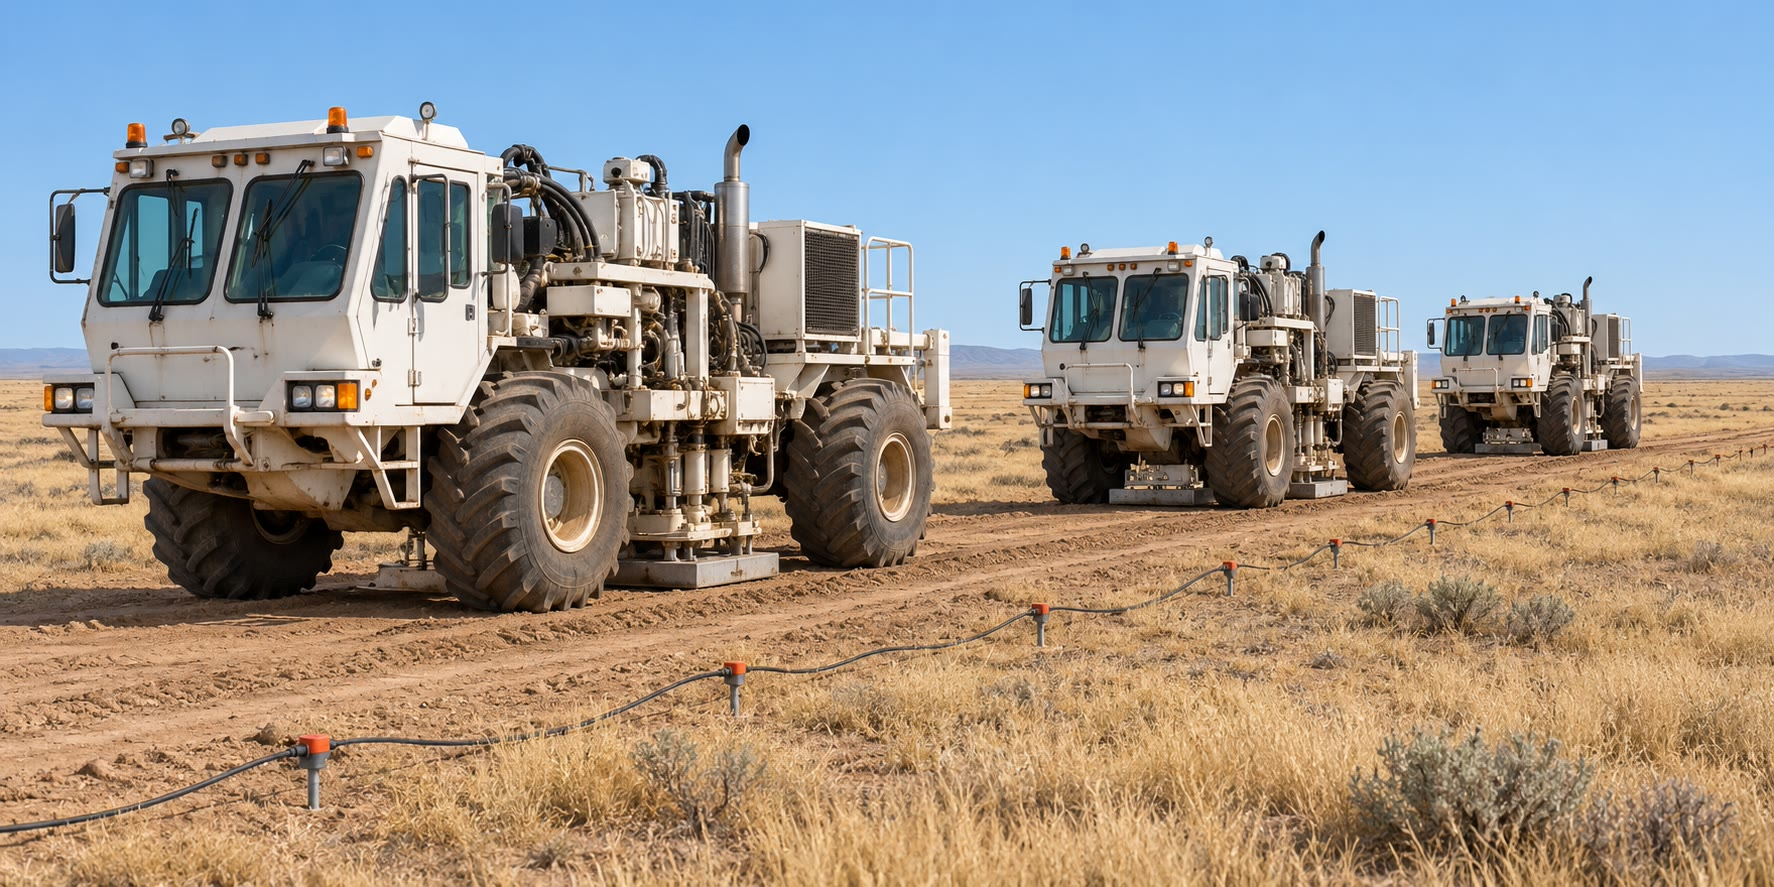
\includegraphics[width=0.62\linewidth]{images/book5/ai/b3-vibroseis.jpg}

\par\smallskip{\small 陆上测线上的震动车：不用爆炸，而是
每辆车将一块重型底板压在地面上，以频率扫描的方式振动数秒；
长记录通过与扫描信号做互相关，压缩为短脉冲，
（AI 生成插图）。}
\label{fig:b3:exploration-seismology:vibroseis}
\end{omfigure}

\section{偏移}

叠加剖面将每个反射显示在记录它的中点之下，
所对应的时间即回波往返所需的时间。对于水平反射面，这一位置是正确的。
对于倾斜反射面则不然：在地表某点记录到的回波，
来自离该点最近的反射面上的点，该点位于上倾方向，
而非正下方。断层切断点等会向各个方向散射能量的点，
在剖面上表现为双曲线。

\begin{definition}[地震偏移]\label{def:b3:exploration-seismology:migration}
\emph{地震偏移}\index{地震偏移}是这样一种处理步骤，
它将地震剖面上的反射移到产生这些反射的反射面位置上：
恢复倾斜反射面的真实倾角与位置，并将点散射体的绕射双曲线
收缩到其顶点处。采用时间域速度模型时，得到时间偏移剖面；
采用深度域模型时，
则得到深度图像。
\end{definition}

\begin{theorem}[零炮检距剖面上的倾角]\label{thm:b3:exploration-seismology:dip}
在速度为 $v$ 的介质中，剖面平面内倾角为 $\theta$ 的平面反射面，
在零炮检距剖面上绘制于各记录点正下方深度 $vt/2$ 处，
表现为视倾角为 $\theta_a$ 的直线，
且满足
\[
  \tan\theta_a = \sin\theta .
\]
在点 $x$ 处记录到的反射，来自反射面上的一点，
该点位于上倾方向，距离为 $(vt/2)\sin\theta$ 处，而非 $x$ 正下方的点。
\end{theorem}

\begin{proof}
零炮检距射线与反射面垂直，因此在 $x$ 处记录的时间为
$t = 2d(x)/v$，其中 $d(x)$ 为 $x$ 到该平面的距离。
沿倾向，距离每增加 $\sin\theta$，$x$ 便移动一个单位，
因此绘制的深度 $vt/2 = d(x)$ 的斜率为 $\sin\theta$。从 $x$ 到该平面的法线垂足
位于水平距离为 $d\sin\theta$ 处，
且在 $x$ 的上倾一侧。
\end{proof}

由于 $\tan\theta_a = \sin\theta < \tan\theta$，未经偏移的剖面总是显示比真实倾角更平缓的倾角，
并且根本无法显示陡于 \ang{45} 的倾角。深度 $z$ 处、位于点 $x_0$ 之下的点散射体，
在 $x$ 处返回的零炮检距时间为 $t(x) = (2/v)\sqrt{z^2 + (x - x_0)^2}$：
这是一条顶点位于该点正上方的双曲线，即绕射。
最简单形式的偏移，即绕射叠加，
沿每个可能散射体的绕射双曲线对剖面求和，并将和置于顶点处：
反射面由连续排列的散射体组成，
它们在其真实位置上显现出来，
而绕射则收缩到各自的顶点。

\begin{omfigure}
\begin{tikzpicture}[font=\small, x=1cm, y=1cm]
\draw[thick] (-0.5,0) -- (8.5,0) node[right] {地表};
% true reflector, dip 35 deg, rising to the left
\draw[very thick, brown!70!black] (1.0,-1.2) -- (6.0,-4.70);
\node[brown!50!black, anchor=east] at (0.95,-1.2) {真实反射面};
% zero-offset normal rays from x = 2, 4, 6
\foreach \x in {2.5, 4.5, 6.5} {
  % distance from (x,0) to the line through (1,-1.2) dir (cos35,-sin35): normal n=(sin35,cos35)
  \pgfmathsetmacro{\dd}{abs(0.5736*(\x-1.0) + 0.8192*(0+1.2))}
  \draw[blue!60!black, ->] (\x,0) -- ++({-0.5736*\dd},{-0.8192*\dd});
  \fill[blue!70!black] (\x,{-\dd}) circle (1.8pt);
}
% apparent reflector through the plotted points
\pgfmathsetmacro{\da}{abs(0.5736*1.5 + 0.8192*1.2)}
\pgfmathsetmacro{\db}{abs(0.5736*5.5 + 0.8192*1.2)}
\draw[blue!70!black, thick, densely dashed] (2.5,{-\da}) -- (6.5,{-\db});
\node[blue!60!black, anchor=west] at (6.6,{-\db}) {未偏移};
\node[anchor=south, font=\scriptsize] at (4.5,0.05) {记录点};
\draw[->, red!70!black, thick] (6.4,{-\db+0.05}) to[bend right=25] ({6.5-0.5736*\db+0.05},{-0.8192*\db-0.12});
\end{tikzpicture}

\par\smallskip{\small 倾斜反射面的偏移（示意图，真实倾角
\ang{35}）。每个记录点处的零偏移距射线垂直于
反射面，因此其回波来自上倾方向；竖直绘于该点正下方，
深度 $vt/2$ 处，反射显得更为平缓（虚线：$\tan\theta_a =
\sin\theta$，此处为 \ang{29.8}），并沿下倾方向发生位移。偏移（红色箭头）将其移回。}
\label{fig:b3:exploration-seismology:migration}
\end{omfigure}

\section{地震地层学}

偏移后的剖面是地层层理的图像，可以按
地层学来解读：反射跟随层面延伸，这些层面
为等时线，因此其几何形态记录了盆地的充填过程。

\begin{definition}[地震地层学，地震相]\label{def:b3:exploration-seismology:seismic-stratigraphy}
\emph{地震地层学}\index{地震地层学}是指根据盆地地震反射的
几何形态，对其地层与沉积历史所作的解释。
\emph{地震相}\index{地震相}是指一个三维反射单元，其
特征（连续性、振幅、
频率、内部几何形态：平行、发散、S 形、杂乱、丘状）
与相邻单元不同，并被解释为一种沉积
环境。
\end{definition}

\begin{definition}[反射终止]\label{def:b3:exploration-seismology:terminations}
\emph{反射终止}\index{反射终止}是指一个反射
与另一反射相接的终点。\emph{上超}\index{上超}：最初水平的反射
终止于一个坡度更陡的面上，较新的地层
超覆于较老的斜坡之上。\emph{下超}\index{下超}：倾斜的
反射沿下倾方向终止于一个更平缓的面上，即进积层
的前端覆于盆地底部。\emph{顶超}\index{顶超}：倾斜的
反射沿上倾方向终止于上覆面，几乎无侵蚀，
进积地层的顶部与海平面相接。\emph{侵蚀
削截}\index{侵蚀削截}：反射沿上倾方向终止于
切割它们的上覆面，即一个不整合。
\end{definition}

\begin{omfigure}
\begin{tikzpicture}[font=\scriptsize, x=1cm, y=1cm]
% erosional truncation: tilted beds cut by an unconformity
\begin{scope}
\foreach \k in {0,...,5} {\draw[gray!60!black] (0,{-2.3+0.32*\k}) -- (3.0,{-1.4+0.32*\k-0.25*0});}
\fill[white] (0,-0.25) -- (3.2,-0.25) -- (3.2,0.4) -- (0,0.4) -- cycle;
\draw[very thick, red!70!black] (0,-0.25) -- (3.0,-0.25);
\foreach \k in {0,1} {\draw[gray!60!black] (0,{-0.05+0.2*\k}) -- (3.0,{-0.05+0.2*\k});}
\node[anchor=north] at (1.5,-2.45) {(a) 侵蚀削截};
\end{scope}
% onlap
\begin{scope}[xshift=3.8cm]
\draw[very thick, red!70!black] (0,-2.3) -- (3.0,-0.2);
\foreach \k in {0,...,5} {\pgfmathsetmacro{\y}{-2.1+0.33*\k} \pgfmathsetmacro{\xe}{(\y+2.3)/0.7} \draw[gray!60!black] (\xe,\y) -- (3.0,\y);}
\node[anchor=north] at (1.5,-2.45) {(b) 上超};
\end{scope}
% downlap and toplap: clinoforms
\begin{scope}[xshift=7.6cm]
\draw[very thick, red!70!black] (0,-2.2) -- (3.6,-2.2);
\draw[very thick, blue!60!black] (0,-0.3) -- (3.6,-0.3);
\foreach \k in {0,...,5} {\draw[gray!60!black] ({0.2+0.5*\k},-0.3) .. controls ({0.7+0.5*\k},-0.4) and ({0.6+0.5*\k},-2.1) .. ({1.1+0.5*\k},-2.2);}
\node[anchor=north] at (1.8,-2.45) {(c) 顶超（顶部），下超（底部）};
\end{scope}
\end{tikzpicture}

\par\smallskip{\small \omterm{def:b3:exploration-seismology:terminations}{反射终止}（示意剖面，灰色为
反射，彩色为终止面）。(a) 倾斜的反射被
不整合切割。(b) 平缓的\omterm{def:b3:exploration-seismology:terminations}{反射终止}于较老的斜坡上。(c) 倾斜的
进积楔地层沿上倾方向终止于其上方的面（\omterm{def:b3:exploration-seismology:terminations}{顶超}），
沿下倾方向终止于盆地底部（\omterm{def:b3:exploration-seismology:terminations}{下超}）。}
\label{fig:b3:exploration-seismology:terminations}
\end{omfigure}

这些终止面界定了成因上相关的地层序列；
在盆地范围内绘制这些终止面，并将其与相对海平面的升降相联系，
即层序地层学，相关内容见
\cref{ch:b3:sequence-stratigraphy}。被动大陆边缘的地震剖面
通常显示向海进积的反射楔，\omterm{def:b3:exploration-seismology:terminations}{下超}于深海
底之上，顶部为\omterm{def:b3:exploration-seismology:terminations}{顶超}，陆向一侧则被海平面
再次上升时沉积的\omterm{def:b3:exploration-seismology:terminations}{上超}地层所掩埋。

\begin{inthefield}[海上拖缆测量与陆上作业队]
\begin{minipage}[t]{0.55\linewidth}\vspace{0pt}
海上测量中，船只从不停下：它沿测线一条接一条地航行，航速只有几节，
气枪阵列以固定间隔激发，拖缆由小型可转向翼片保持在
恒定深度，并通过声学和卫星定位
进行定位。驾驶台上的观测员监视阵列周围的海面，并且
测量须遵守相关规定，其中列明了保护海洋哺乳动物的措施、
值守的要求以及须上报的事项。
% ledger: noaa5:itr-gom
在陆地上，作业队沿测线布设电缆或无线记录单元；
可控震源车成队从一个震源点推进到下一个，而
记录车在每次扫描前检查每个道。回到处理中心后，
记录被整理为\omterm{def:b3:exploration-seismology:cmp}{共中心点}道集，速度
被拾取，数据经过叠加和偏移，剖面交给
解释人员。
\end{minipage}\hfill
\begin{minipage}[t]{0.42\linewidth}\vspace{0pt}
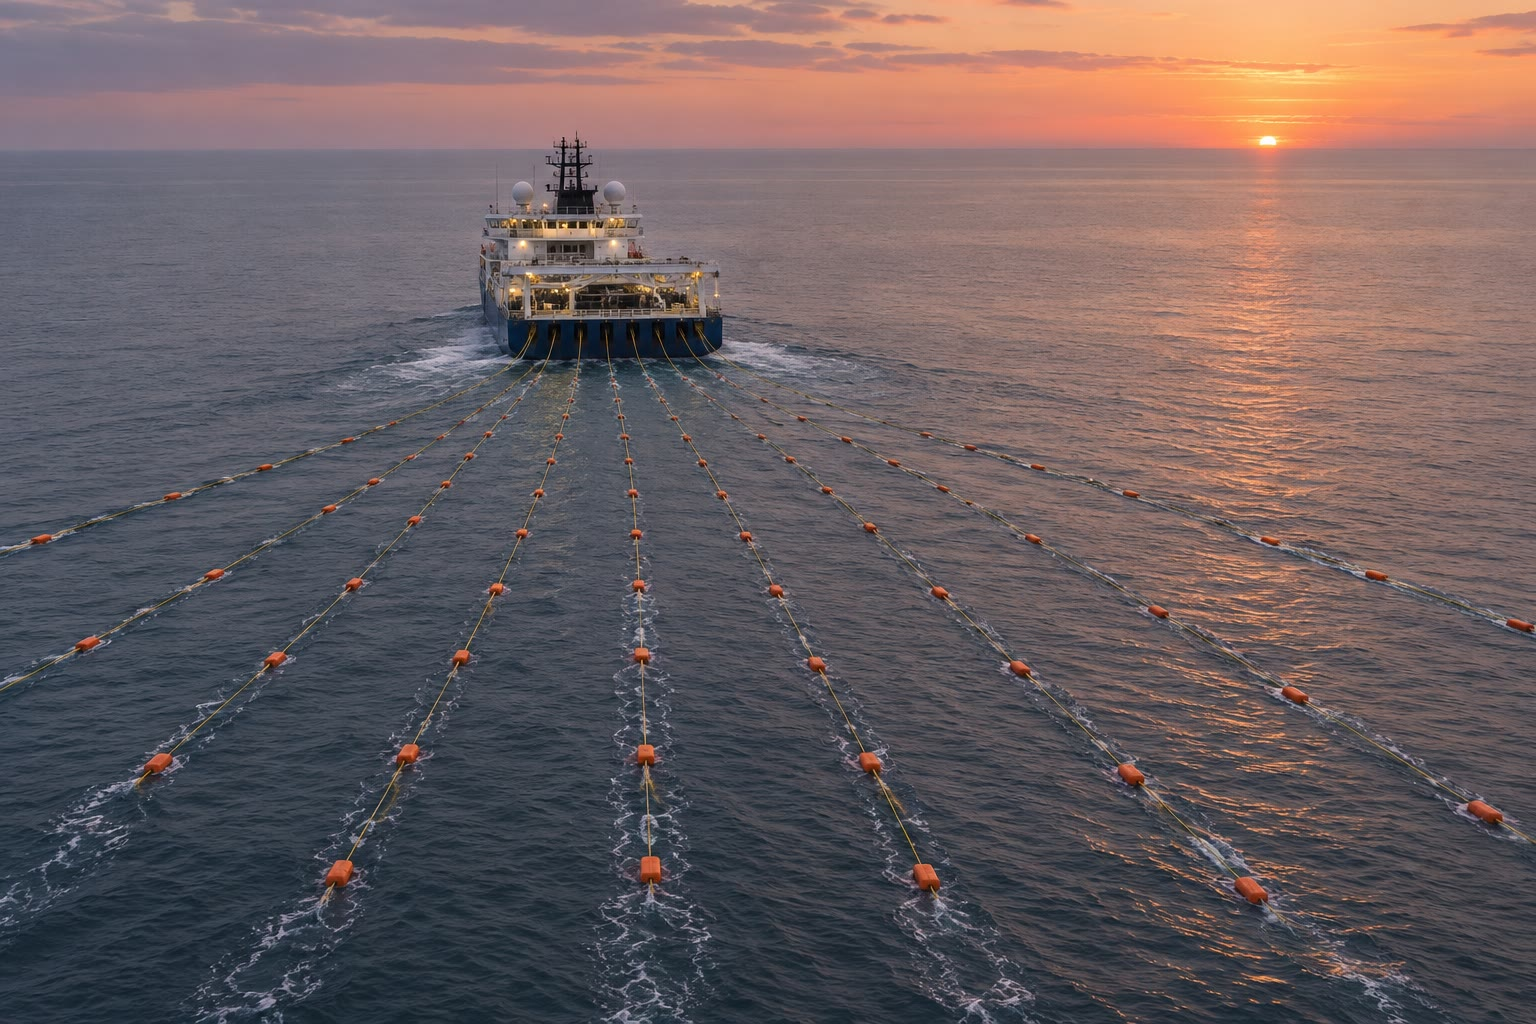
\includegraphics[width=\linewidth]{images/book5/ai/b3-streamer-vessel.jpg}

{\scriptsize 黄昏时拖着拖缆航行的地震测量船
（AI 生成插图）。}
\end{minipage}
\end{inthefield}

\section{练习}

\begin{exercise}[$\star$]\label{exo:b3:exploration-seismology:1}
白垩（$v = \qty{2500}{m.s^{-1}}$，$\rho = \qty{2.00}{g.cm^{-3}}$）位于页岩
（\qty{2300}{m.s^{-1}}，\qty{2.30}{g.cm^{-3}}）之上，页岩又位于石灰岩
（\qty{4500}{m.s^{-1}}，\qty{2.60}{g.cm^{-3}}）之上。计算三种阻抗以及
两个界面的反射系数。
石灰岩顶面反射的入射能量占多大比例？
% ledger: mavko:velocities
\end{exercise}

\begin{exercise}[$\star$]\label{exo:b3:exploration-seismology:2}
水平反射面位于速度为\qty{2000}{m.s^{-1}}的层之下\qty{800}{m}处。
计算 $t_0$、炮检距为\qty{1000}{m}处的反射时间，以及该处的
\omterm{thm:b3:exploration-seismology:nmo}{正常时差}，并与近似式 $x^2/(2v^2t_0)$ 比较。
\end{exercise}

\begin{exercise}[$\star$]\label{exo:b3:exploration-seismology:3}
一根拖缆上有 240 道，道间距为\qty{12.5}{m}，船每隔
\qty{25}{m}激发一次。计算\omterm{def:b3:exploration-seismology:cmp}{共中心点}间距与\omterm{def:b3:exploration-seismology:cmp}{覆盖次数}。
若要使\omterm{def:b3:exploration-seismology:cmp}{覆盖次数}为 120，炮间距应为多少？
\end{exercise}

\begin{exercise}[$\star$]\label{exo:b3:exploration-seismology:4}
主频为\qty{30}{Hz}时，计算波长及
四分之一波长（砂岩中，速度为\qty{3000}{m.s^{-1}}；石灰岩中，速度为
\qty{4500}{m.s^{-1}}）。计算一反射面的第一\omterm{def:b3:exploration-seismology:fresnel}{菲涅耳带}半径，
该反射面埋深\qty{1000}{m}，上覆岩石平均速度为\qty{2800}{m.s^{-1}}。
\end{exercise}

\begin{exercise}[$\star\star$]\label{exo:b3:exploration-seismology:5}
两个反射中，一个 $t_0 = \qty{0.500}{s}$，其\omterm{def:b3:exploration-seismology:velocities}{均方根速度}为
\qty{2400}{m.s^{-1}}，另一反射的 $t_0 = \qty{0.700}{s}$，其\omterm{def:b3:exploration-seismology:velocities}{均方根速度}为\qty{2800}{m.s^{-1}}。
计算\omterm{def:b3:exploration-seismology:velocities}{层速度}及两者之间该层的厚度。
\end{exercise}

\begin{exercise}[$\star\star$]\label{exo:b3:exploration-seismology:6}
设一平面反射面在\omterm{def:b3:exploration-seismology:cmp}{共中心点}测线所在平面内的倾角为 $\varphi$，位于
速度为 $v$ 的层中。（a）证明 $t(x)^2 = t_0^2 + x^2\cos^2\varphi/v^2$，其中 $t_0$ 为
中心点处的零炮检距时间。（提示：利用中心点关于
反射面的镜像。）（b）推出\omterm{def:b3:exploration-seismology:velocities}{叠加速度}，并在
$v = \qty{2000}{m.s^{-1}}$、$\varphi = \ang{12}$ 时计算其值。
\end{exercise}

\begin{exercise}[$\star\star$]\label{exo:b3:exploration-seismology:7}
\omterm{def:b3:exploration-seismology:cmp}{覆盖次数}为 60 的道集，各道上噪声相互独立且方差相同。
叠加使信噪比提高到原来的多少倍？再使其加倍，\omterm{def:b3:exploration-seismology:cmp}{覆盖次数}
须增加为原来的多少倍？
\end{exercise}

\begin{exercise}[$\star\star$]\label{exo:b3:exploration-seismology:8}
在速度为\qty{3000}{m.s^{-1}}的岩石中，零炮检距时间剖面上的一个反射
沿测线每千米双程时抬升\qty{0.40}{s}。将此斜率换算为
视倾角，并计算反射面的真倾角。
\end{exercise}

\begin{exercise}[$\star\star$]\label{exo:b3:exploration-seismology:9}
将\omterm{def:b3:exploration-seismology:synthetic}{反射系数序列} $r = (0, 0.3, 0, -0.2, 0)$ 与
三样本子波 $w = (-0.5, 1, -0.5)$，逐样本卷积。两个
反射位于何处？它们是否重叠？
\end{exercise}

\begin{exercise}[$\star\star\star$]\label{exo:b3:exploration-seismology:10}
在速度为\qty{1800}{m.s^{-1}}的层上作反向折射剖面，得到
沿下倾方向的视速度为\qty{2900}{m.s^{-1}}，沿上倾方向的
视速度为\qty{4400}{m.s^{-1}}。计算临界角、倾角及
折射\omterm{def:b3:exploration-seismology:velocities}{层速度}，并将其与两个视速度的
调和平均值相比较。
\end{exercise}

\begin{exercise}[$\star\star\star$]\label{exo:b3:exploration-seismology:11}
在\cref{prop:b3:exploration-seismology:tuning}中，某层的反射系数为
$+R$ 与 $-R$。（a）证明：当 $\Delta t \ll T$ 时，复合信号
近似为 $R\,\Delta t\,w'(t)$，即子波对时间的导数，
再乘以该层的双程厚度。（b）说明薄层虽不能分辨，却仍能被
探测到，并说明如何由其振幅估计厚度。（c）同种岩石的两层，
厚度分别为 5 和\qty{10}{m}，以相同子波成像，
二者振幅之比为多少？
\end{exercise}

\begin{exercise}[$\star\star\star$]\label{exo:b3:exploration-seismology:12}
一点散射体位于测线下方\qty{600}{m}处，岩石速度为
\qty{3000}{m.s^{-1}}。（a）写出该绕射的零炮检距时间
关于水平距离 $x$（自其正上方的点量起）的表达式，并计算 $x = 0$
与\qty{300}{m}处的值。（b）证明该绕射为\omterm{thm:b3:exploration-seismology:nmo}{正常时差}形式的
双曲线，速度为 $v/2$，并说明在顶点时间相同时，绕射总比
同顶点时间的反射更弯曲。（c）偏移对它有何作用？
\end{exercise}

\section{问题：横穿瓦尔登丘陵的地震测线}

\begin{problem}[{周末问题——折射、速度分析、深度
转换与沿瓦尔登丘陵 A--B 剖面的偏移}]
\label{pb:b3:exploration-seismology:1}
% values: calc/ch02.py, from figdata seismic_model.py, refraction_dip.py, cmp_nmo.py
地震测线沿瓦尔登丘陵的 A--B 剖面布设，该剖面位于
前几册地质图所示的区域内。测线距离 $s$ 自
A 沿测线起算。自上而下，覆盖层依次为白垩、页岩（\qty{100}{m}）、
石灰岩（\qty{180}{m}）与砂岩（\qty{120}{m}），以不整合形式覆于
片岩基底之上；覆盖层被褶皱成一背斜和一向斜，并被一条
正断层切割。

\medskip
\noindent\textbf{第一部分——西翼上的折射排列。}一条
长\qty{1200}{m}的观测排列布设于炮点 W（$s = \qty{300}{m}$）与
E（$s = \qty{1500}{m}$）之间，地面视为水平。石灰岩以上的白垩与页岩
合并视为一层，速度 $v_1 = \qty{2.40}{km.s^{-1}}$。
记录上读得的首波走时，自 W 向 E 时，\qty{425.2}{ms}对应
\qty{800}{m}，\qty{486.1}{ms}对应\qty{1200}{m}；自 E 向 W 时，
\qty{372.4}{ms}对应\qty{800}{m}，\qty{486.1}{ms}对应\qty{1200}{m}。
\begin{enumerate}
  \item 计算两个视速度。哪一炮点位于上倾方向？
  \item 计算临界角及折射层的倾角。
  \item 计算折射层的速度，它是何种岩石？
  \item 计算截距时间，以及折射层在
        W 和 E 下方的法向深度。
  \item 将其换算为铅直深度，并由两个深度检验倾角。
  \item 白垩之下的页岩比白垩慢。折射测量对此
        会作何解释，它又如何使深度产生偏差？
\end{enumerate}

\noindent\textbf{第二部分——CMP S 处的速度分析。}更靠东的 CMP S
位于向斜轴上，处于断层的下降盘，此处各层
视为水平。拾取四个反射在零炮检距及
\qty{600}{m}处的走时：
\begin{center}
\small
\begin{tabular}{lcccc}
\hline
反射 & 1 & 2 & 3 & 4 \\
$t_0$ (\unit{s}) & 0.4878 & 0.5748 & 0.6548 & 0.7348 \\
$t(\qty{600}{m})$ (\unit{s}) & 0.5437 & 0.6240 & 0.6887 & 0.7648 \\
\hline
\end{tabular}
\end{center}
\begin{enumerate}[resume]
  \item 计算反射 1 的 NMO 速度 $V = x/\sqrt{t^2 - t_0^2}$，
        及反射 2 的 NMO 速度。为何第二个比第一个小？
  \item 计算反射 3 和 4 的 NMO 速度。
  \item 将这些速度取为\omterm{def:b3:exploration-seismology:velocities}{均方根速度}，由\omterm{thm:b3:exploration-seismology:dix}{迪克斯公式}
        计算各层的\omterm{def:b3:exploration-seismology:velocities}{层速度}。
  \item 根据速度判断各层为何种岩石，并命名
        四个反射界面。
  \item 反射 1 在记录上最弱，为什么？
  \item 为何速度只在炮检距至 \qty{600}{m}
        的范围内测量，而排列长度达 \qty{2}{km}？
\end{enumerate}

\noindent\textbf{第三部分——深度转换与分辨率。}
\begin{enumerate}[resume]
  \item 计算每层中的双程走时及其厚度。
  \item 计算各反射界面在地面以下的深度。比较
        页岩、石灰岩和砂岩的厚度与上文
        给出的数值。
  \item 计算从地面到基底的平均速度，并说明为何
        若改用反射 4 的 NMO 速度，
        则会高估深度。
  \item 测得\omterm{def:b3:exploration-seismology:wavelet}{地震子波}的峰值频率为 \qty{30}{Hz}。计算页岩中的波长
        及其\omterm{def:b3:exploration-seismology:resolution}{调谐厚度}，分别用四分之一波长法则
        和\omterm{def:b3:exploration-seismology:wavelet}{里克子波}的 $b = v/(5.2f)$ 方法计算。页岩能否被分辨？
        按四分之一波长法则，频率为多少时页岩会发生调谐？
  \item 计算基底上第一\omterm{def:b3:exploration-seismology:fresnel}{菲涅耳带}的半径，取
        $\lambda$ 由反射 4 的 NMO 速度确定。
\end{enumerate}

\noindent\textbf{第四部分——偏移与断层。}
\begin{enumerate}[resume]
  \item 在断层附近，石灰岩的截断产生一个绕射，
        其顶点位于 \qty{0.550}{s}；沿测线距顶点 \qty{200}{m} 处，
        其走时为 \qty{0.5732}{s}。写出零炮检距绕射走时，
        并推算截断面以上的平均速度。
  \item 计算截断点在地面以下的深度。
  \item 在东翼，叠加剖面上石灰岩顶面的反射
        向背斜方向抬升，每千米双程走时
        减少 \qty{0.167}{s}，岩层平均速度为 \qty{2.48}{km.s^{-1}}。计算其
        视倾角及真倾角。
  \item 该翼上某一反射的记录时间为 $t = \qty{0.655}{s}$。偏移将其移动多远，
        并沿何方向移动？
  \item 穿过断层时，基底顶面的反射跳跃 \qty{0.160}{s}；
        下降盘中白垩层增加了额外厚度。计算
        垂直断距。
  \item 根据第二部分的\omterm{def:b3:exploration-seismology:velocities}{层速度}，求出
        基底不整合在 CMP S 之下的深度。
\end{enumerate}
\end{problem}
